% EXPANDED RESEARCH PAPER 2026-10-30
% ABSTRACT START
\noindent\textbf{Abstract---}
Automatic sentiment classification can support the analysis of product reviews, but reported differences between neural architectures are difficult to interpret when datasets and evaluation procedures vary. This study compares a multi-layer perceptron (MLP) operating on term frequency--inverse document frequency features, a convolutional text classifier (TextCNN), and a bidirectional long short-term memory network (BiLSTM) under a shared experimental protocol. A balanced subset of 20,000 real Amazon Polarity reviews is cleaned once and divided into stratified training, validation, and test partitions of 16,000, 2,000, and 2,000 reviews. Two configurations per architecture are compared using validation loss, with early stopping and best-checkpoint selection preceding test evaluation. The MLP achieves the highest test accuracy of 88.20\% and positive-class F1-score of 0.8829, followed by BiLSTM at 86.10\% and 0.8614, and TextCNN at 85.40\% and 0.8576. Batched data loading and sparse feature storage enable the complete experiment to run on a local CPU with a maximum recorded worker-process-tree private memory of 686.5 MiB. Analysis of real misclassifications identifies difficulties involving negation, mixed opinions, ironic praise, and opinion targets, alongside possible label inconsistency. The findings support a strong sparse-feature baseline in this setting while emphasizing the limitations of a single-seed comparison and truncated sequence inputs.
% ABSTRACT END

\par\vspace{4pt}
{\raggedright\noindent\textit{Keywords---}sentiment analysis, Amazon Polarity, product reviews, deep learning, TF-IDF, multi-layer perceptron, TextCNN, bidirectional LSTM\par}

\section{Introduction}
Online product reviews express customer experiences with quality, reliability, usability, and service. Their volume makes exhaustive manual analysis difficult, motivating automated classification of review polarity. Early supervised sentiment-classification research established that the task requires more than counting apparently positive and negative words: the interpretation of an expression depends on its context and the object being evaluated~\cite{pang2002}. Large product-review benchmarks subsequently enabled systematic evaluation of text classifiers at substantially greater scale~\cite{zhang2015}.

Three architecture families provide a useful comparison within an undergraduate deep-learning project. A feed-forward classifier can combine sparse lexical evidence, a convolutional classifier can detect local patterns~\cite{kim2014}, and a recurrent classifier can represent sequential dependencies~\cite{hochreiter1997}. Bidirectional recurrence extends the latter by processing the observed sequence in both directions~\cite{schuster1997}. Pretrained Transformer models, including BERT~\cite{devlin2019}, provide a broader research context, but are outside this project's three-model scope.

This paper compares an MLP using TF-IDF features, a TextCNN using learned word embeddings, and a BiLSTM using the same tokenized sequences as the TextCNN. All three models use the same source reviews, cleaning procedure, labels, stratified partitions, and evaluation metrics. Input representation differs deliberately: the MLP receives lexical features from the complete cleaned review, whereas the two sequence models receive at most 100 tokens. Consequently, the experiment compares architecture--representation configurations rather than isolating architecture from every other factor.

The study addresses two practical concerns. First, small neural classifiers can overfit a limited labeled subset despite a large underlying corpus; validation-based selection is therefore essential. Second, converting millions of review strings or an entire TF-IDF matrix into dense in-memory representations can make an otherwise modest experiment infeasible. A memory-conscious pipeline is used to complete the comparison and preserve predictions for subsequent error analysis. The contribution is an auditable comparison under a common protocol, accompanied by an interpretation of performance differences and concrete failure cases.


Three research questions guide the analysis. RQ1 asks which of the three specified configurations gives the strongest observed held-out classification performance under a shared data and tuning budget. RQ2 asks what the validation trajectories and resource measurements reveal about the practical costs of obtaining that performance. RQ3 asks which kinds of review interpretation remain difficult across configurations. These questions separate a quantitative comparison from qualitative explanations: a higher score answers the first question for this run, while a plausible account of a failure remains a hypothesis requiring further controlled evaluation.

The unit of prediction is the review formed by joining its title and content. The target is the binary source polarity, rather than an aspect-specific opinion, a star-rating regression target, or a verified statement about product quality. A review may praise one feature and criticize another while still carrying a single document label. This distinction matters because successful polarity prediction does not establish that a model identifies the correct opinion target or supports a factual claim about the product. The experiment measures agreement with corpus labels and examines the boundaries of that agreement.


\section{Literature Review}
\subsection{Sentiment representations and shallow classifiers}
Pang, Lee, and Vaithyanathan~\cite{pang2002} examined supervised document-level sentiment classification, establishing an influential baseline for learning polarity from lexical features. Maas et al.~\cite{maas2011} combined representation learning with sentiment supervision and introduced the widely used IMDB movie-review benchmark. Although that corpus is outside the present product-review scope, it demonstrates the importance of separating evaluation domains and protocols. Mikolov et al.~\cite{mikolov2013} developed efficient distributed word representations using skip-gram improvements and negative sampling, motivating the use of embedding-based inputs in neural text classification. The embeddings in this project are learned from the training subset rather than imported from that pretrained representation.

Joulin et al.~\cite{joulin2017} showed that efficient classifiers based on word and n-gram representations can remain competitive with more elaborate text models. This finding motivates retaining a strong lexical baseline rather than assuming that greater sequential complexity must improve accuracy. Our MLP is not fastText: it operates on TF-IDF features and contains two nonlinear hidden layers. The connection is the value of inexpensive lexical representations as a reference point for neural comparisons.

\subsection{Convolutional and compositional models}
Kim~\cite{kim2014} demonstrated the effectiveness of convolution and max-over-time pooling over word vectors for sentence classification. The present TextCNN follows that general pattern but uses one filter width and randomly initialized, trainable embeddings. Zhang, Zhao, and LeCun~\cite{zhang2015} investigated character-level convolutional classifiers and introduced large text-classification datasets, including Amazon review polarity. Their character-based model differs from the word-level convolution used here; their work supplies the dataset context rather than an identical model specification.

Socher et al.~\cite{socher2013} studied semantic composition using a recursive neural tensor network and the Stanford Sentiment Treebank. Their treatment of compositional sentiment provides a motivation for examining negation and apparently conflicting polarity cues. The present classifiers do not use syntactic parse trees or phrase-level sentiment labels, so similar linguistic phenomena must be learned indirectly from review-level supervision.

\subsection{Recurrent and attention-based models}
Hochreiter and Schmidhuber~\cite{hochreiter1997} introduced LSTM memory cells to address difficulties in learning dependencies across long sequences. Schuster and Paliwal~\cite{schuster1997} developed bidirectional recurrent networks that incorporate context from both sequence directions. These ideas motivate the BiLSTM architecture, although its accessible context in this experiment is restricted to the first 100 tokens of each review. Zhou et al.~\cite{zhou2016} combined bidirectional LSTM representations with attention for relation classification. Because that task and dataset differ from review-polarity classification, the work is relevant as an architectural extension rather than as a directly comparable sentiment benchmark.

Vaswani et al.~\cite{vaswani2017} introduced the Transformer architecture, and Devlin et al.~\cite{devlin2019} demonstrated the value of pretrained bidirectional Transformer representations for language understanding. These works indicate a direction for future comparison, but no Transformer result is claimed in this study. Collectively, the reviewed literature motivates the selected feed-forward, convolutional, and recurrent families while underscoring why results reported under different data and training conditions should not be treated as a controlled ranking.


\subsection{Position of the present comparison}
The reviewed methods differ in supervision, input granularity, pretrained resources, and evaluation domain. Table~\ref{tab:literature} maps those differences to this experiment. Published benchmark scores are not reproduced as a league table because such numbers would combine incompatible datasets and training budgets. The present study instead holds review identities and evaluation rules fixed and explicitly records the remaining representation differences.

\begin{table*}[tbp]
\fontsize{9}{10.2}\selectfont
\centering
\caption{Relationship Between Prior Methods and the Present Study}
\label{tab:literature}
\renewcommand{\arraystretch}{1.10}\setlength{\tabcolsep}{4pt}
\begin{tabularx}{\linewidth}{@{}P{32mm}P{48mm}Y@{}}
\toprule
Research & Relevant idea & Boundary of comparison \\ \midrule
Pang et al.~\cite{pang2002}; Joulin et al.~\cite{joulin2017} & Lexical and n-gram evidence for document classification & Our lexical classifier is a nonlinear TF-IDF MLP, not an implementation of either published system. \\
Kim~\cite{kim2014} & Convolution with max-over-time pooling & We use one filter width and train embeddings from scratch on review-level labels. \\
Socher et al.~\cite{socher2013} & Compositional interpretation of sentiment & No parse trees or phrase-level labels are available to our classifiers. \\
Hochreiter and Schmidhuber~\cite{hochreiter1997}; Schuster and Paliwal~\cite{schuster1997} & Gated recurrence and bidirectional context & Context is restricted to the retained 100-token sequence. \\
Zhou et al.~\cite{zhou2016} & Attention over bidirectional states & Relation classification motivates an extension; attention is not evaluated here. \\
Vaswani et al.~\cite{vaswani2017}; Devlin et al.~\cite{devlin2019} & Attention and pretrained contextual representations & Transformer training and pretrained resources lie outside the reported experiments. \\
\bottomrule
\end{tabularx}
\end{table*}

The resulting research gap is local and practical: how these three accessible configurations behave on a fixed, modest product-review subset when training and validation controls are made explicit. The contribution is not a new neural layer or a state-of-the-art claim. It is an evidence-linked comparison that includes error behavior, input coverage, and implementation cost alongside aggregate predictive scores.


\section{Objectives}
\begin{enumerate}
\item Compare MLP, TextCNN, and BiLSTM on the same 20,000-review Amazon Polarity subset and held-out test partition using accuracy, precision, recall, and F1-score.
\item Interpret observed performance differences through the models' representations, architectural properties, validation trajectories, and sequence-length limitations.
\item Identify recurring classification difficulties by examining exported misclassifications and reviewed examples of negation, mixed sentiment, ironic praise, and differing opinion targets.
\end{enumerate}

\section{Methodology}
Each classifier produces a positive-class probability $p_\theta(x)$ through a sigmoid output. The predicted label is $\widehat y=\mathbf{1}[p_\theta(x)>0.5]$, with label 1 denoting positive sentiment and label 0 negative sentiment. The common optimization objective is binary cross-entropy,
\begin{equation}
\begin{aligned}
\mathcal{L}(\theta)=-\frac{1}{N}\sum_{i=1}^{N}\bigl[&
y_i\log p_\theta(x_i)\\
&+(1-y_i)\log(1-p_\theta(x_i))\bigr].
\end{aligned}
\end{equation}
Dropout is used to reduce co-adaptation during training~\cite{srivastava2014}. All models use Adam~\cite{kingma2015} with a weight-decay coefficient of $10^{-4}$; decoupled weight decay provides a relevant regularization principle for adaptive optimization~\cite{loshchilov2019}. Table~\ref{tab:architectures} summarizes the implemented architectures. Configuration selection and stopping rules are specified in Section~\ref{sec:setup}.

\begin{table*}[tbp]
\fontsize{9}{10.2}\selectfont
\centering
\caption{Model Architectures and Trainable Parameter Counts}
\label{tab:architectures}
\setlength{\tabcolsep}{4pt}\renewcommand{\arraystretch}{1.12}
\begin{tabularx}{\linewidth}{@{}P{17mm}P{39mm}Y r@{}}
\toprule
Model & Representation & Network after representation & Parameters \\ \midrule
MLP & TF-IDF, up to 20,000 unigrams/bigrams & Dense 256; dropout; Dense 64; dropout; sigmoid & 5,136,769 \\
TextCNN & 100 token IDs; 100-dimensional embeddings & Conv1D 128, width 5; max pooling; Dense 64; dropout; sigmoid & 2,072,449 \\
BiLSTM & Same token IDs and embedding dimension & Bidirectional LSTM 64; Dense 64; dropout; sigmoid & 2,092,801 \\
\bottomrule
\end{tabularx}
\end{table*}


\begin{figure*}[tbp]
\centering
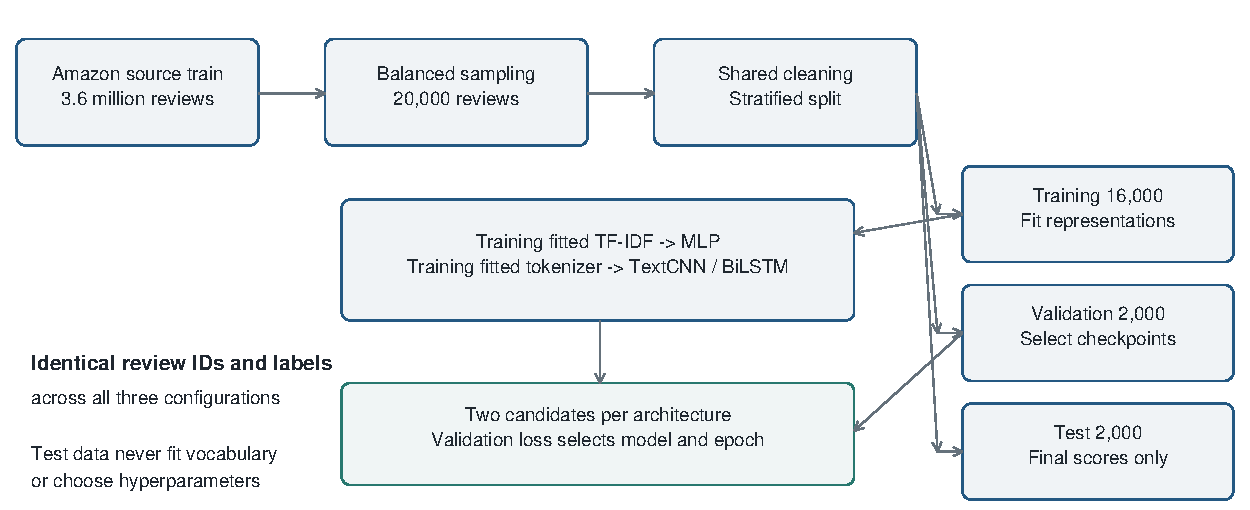
\includegraphics[width=0.80\textwidth]{figures/experiment_workflow.pdf}
\caption{Shared experimental workflow. Only training reviews fit the feature representations. Validation loss selects candidates and checkpoints; the test partition is reserved for evaluation after selection.}
\label{fig:workflow}
\end{figure*}

Figure~\ref{fig:workflow} separates three operations that can otherwise be conflated: learning the input representation, fitting network parameters, and selecting a configuration. The first two use the training partition; the third uses validation loss. Transforming a held-out review with an already fitted vectorizer is permitted, whereas allowing that review to change vocabulary weights would leak information across this boundary. The fixed threshold is not tuned on test outcomes.

\begin{figure*}[tbp]
\centering
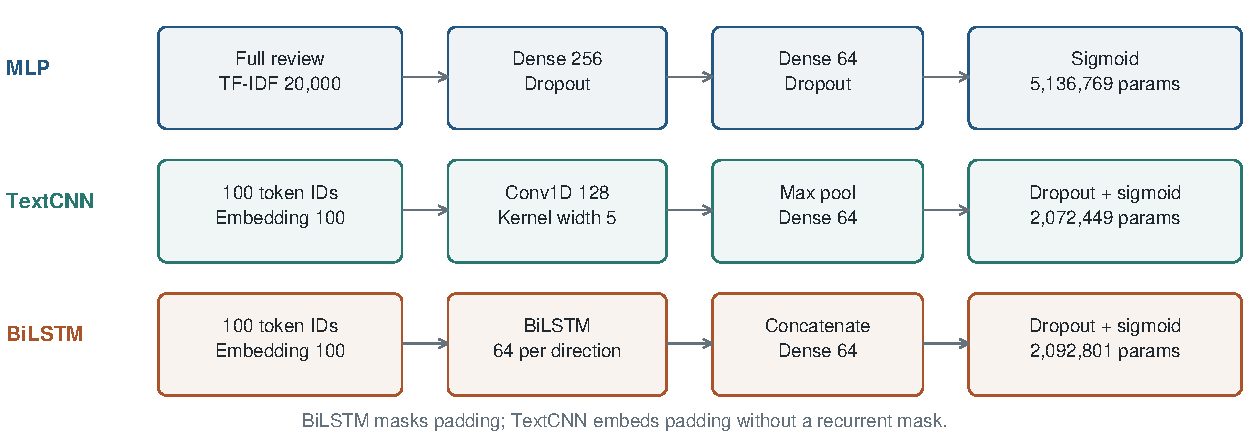
\includegraphics[width=0.80\textwidth]{figures/model_architectures.pdf}
\caption{Implemented computation paths. Dense sizes, convolutional settings, recurrent units, and parameter counts correspond to the saved model specifications. Embedding dimension is 100 for both sequence models.}
\label{fig:architectures}
\end{figure*}

Figure~\ref{fig:architectures} shows where the configurations differ. The MLP spends most parameters on the input projection. Both sequence models allocate two million parameters to their embedding tables before their convolutional or recurrent encoders. Parameter count therefore describes the implemented capacity but is not a direct measure of computation per example or the amount of linguistic context available.


\subsection{MLP on TF-IDF Features}
The MLP baseline, assigned to Pankhuri Kumari, represents each cleaned review using TF-IDF-weighted unigrams and bigrams. The feature vocabulary is fitted exclusively on training reviews and capped at 20,000 terms. With $N$ training documents and document frequency $\operatorname{df}(t)$, the smoothed inverse document frequency is
\begin{equation}
\operatorname{idf}(t)=\log\frac{1+N}{1+\operatorname{df}(t)}+1.
\end{equation}
Term counts are multiplied by this weight and each document vector is normalized to unit Euclidean length. Features remain in float32 compressed sparse row (CSR) form between batches.

The network contains hidden layers of 256 and 64 rectified linear units, each followed by dropout, and a single sigmoid output. This architecture serves as the feed-forward reference: it can combine evidence from the full review but represents word order only indirectly through bigram features. Its larger parameter count primarily reflects the first dense transformation from the high-dimensional lexical input. The selected configuration uses dropout 0.5 and learning rate $5\times10^{-4}$.


For a normalized feature vector $v$, the feed-forward computation is
\begin{equation}
\begin{aligned}
h_1&=\operatorname{ReLU}(W_1v+b_1),\\
h_2&=\operatorname{ReLU}(W_2\widetilde h_1+b_2),\\
p&=\sigma(w_o^\top\widetilde h_2+b_o),
\end{aligned}
\end{equation}
where tildes denote dropout during training; inference uses the learned deterministic network. The first layer alone contains $20{,}000\times256+256=5{,}120{,}256$ parameters, accounting for approximately 99.68\% of the complete MLP. Its apparently larger model size is thus mostly a consequence of lexical input dimensionality.

TF-IDF retains evidence from a word wherever it occurs in the review, and bigrams capture some local order. It does not retain an unrestricted sequence of clauses or explicitly bind an opinion to a product aspect. If favorable and unfavorable phrases occur together, the hidden layers must learn how their aggregate feature pattern corresponds to the document label. This explains what information is available to the classifier without asserting which features caused any particular prediction.


\subsection{TextCNN on Learned Word Embeddings}
The TextCNN, assigned to Sai Prasad Prusty, receives integer sequences generated by a training-only tokenizer. Reviews are truncated or post-padded to 100 tokens. The vocabulary is capped at 20,000 entries and includes an out-of-vocabulary token. A trainable embedding layer maps each token to a 100-dimensional vector. A one-dimensional convolution applies 128 filters of width 5, followed by ReLU activation and global max pooling. The pooled representation passes through a 64-unit ReLU layer, dropout, and the sigmoid output.

For a filter applied at position $i$, a local activation can be expressed as $c_i=\operatorname{ReLU}(W[e_i;\ldots;e_{i+4}]+b)$; max pooling retains its strongest response over the observed sequence. This mechanism motivates the model's capacity to recognize local sentiment patterns. It does not guarantee correct treatment of negation or sarcasm. The selected configuration uses dropout 0.3 and learning rate $10^{-3}$. Unlike the pretrained-vector variants studied by Kim~\cite{kim2014}, all embeddings are learned from this project's training subset.


With valid convolution, a 100-token input and width-five kernel produce 96 positions per filter. Max pooling reduces those positions to one value for each of the 128 filters, yielding a fixed-size representation independent of the number of unpadded tokens. This reduction makes a strong local activation easy to propagate to the output, but discards its exact position and does not explicitly encode the relation between two distant clauses.

The embedding layer in this TextCNN does not mask zero padding. Consequently, post-padding is processed by the embedding and convolution operations, unlike the explicitly masked BiLSTM input. This is an implementation difference in addition to the distinction between convolution and recurrence. A padding-aware pooling or convolution variant would be a useful controlled extension, but its effect cannot be inferred from the present scores.


\subsection{BiLSTM on the Shared Sequence Representation}
The BiLSTM, assigned to Jambhorkar Arya Sachin, uses the same tokenizer, sequence length, and embedding dimension as the TextCNN. It contains 64 LSTM units in each direction. The final forward and backward representations are concatenated and passed through a 64-unit ReLU layer, dropout, and a sigmoid output. Zero-valued padding tokens are masked, preventing them from being treated as ordinary review words by the recurrent layer.

Bidirectional processing is included to model order and contextual dependencies within the retained sequence. Its potential advantage over convolution is therefore contextual rather than an ability to observe the entire original review: both sequence models remain subject to the same 100-token truncation. The selected BiLSTM uses dropout 0.3 and learning rate $10^{-3}$. No attention mechanism or pretrained embeddings are included, preserving the intended comparison of the three specified architecture families.


For the retained embeddings $e_1,\ldots,e_T$, bidirectional recurrence computes
\begin{equation}
\begin{aligned}
\overrightarrow h_t&=\operatorname{LSTM}_f(e_t,\overrightarrow h_{t-1}),\\
\overleftarrow h_t&=\operatorname{LSTM}_b(e_t,\overleftarrow h_{t+1}).
\end{aligned}
\end{equation}
The classifier uses the final states from the forward and backward passes as its 128-dimensional encoded representation. Both directions observe the same retained prefix; reading this prefix backward does not recover discarded tokens. The recurrent encoder has 84,480 parameters across the two directions, while its embedding table contains 2,000,000. These counts distinguish the role of representation storage from the cost of repeated state updates.

Masking prevents padding tokens from advancing the recurrent interpretation as ordinary review words. It does not supply a missing conclusion, correct a mislabeled document, or make a domain-specific expression unambiguous. For example, a final recommendation beyond token 100 is unavailable regardless of the recurrent cell's nominal ability to preserve long-term dependencies.


\section{Experimental Setup}\label{sec:setup}
The final experiment extends the Phase 2 interim implementation with validation-based early stopping, checkpoint selection, and a bounded tuning search. Embedding dimensions, convolutional filter settings, and recurrent-unit counts remain fixed; tuning covers two dropout/learning-rate pairs with a common weight-decay coefficient. Execution uses a local CPU in place of the Colab environment envisaged in the synopsis. The interim report's preliminary five-epoch scores are superseded by the audited final run reported here. Because the data-processing and training pipeline was revised, differences from the interim scores do not constitute a controlled ablation of regularization.

\subsection{Dataset and Shared Partitions}
The experiment uses the training partition of the publicly available Amazon Polarity dataset~\cite{zhang2015}, pinned to Hugging Face revision 9d9c45c18f8c3cf1b23a3c27917b60cbf28f3289. Its 3.6 million source training rows are scanned through parquet batches. Label-wise sampling without replacement uses seed 42, with deterministic reserves to replace empty, duplicate, or conflicting cleaned texts. The resulting subset contains exactly 10,000 positive and 10,000 negative reviews. No duplicate or conflicting cleaned text was found among this run's 22,000 sampled candidates.

The subset is stratified into 16,000 training, 2,000 validation, and 2,000 test reviews, with equal class counts in every partition. Source review identifiers and cleaned texts are checked for overlap across partitions. All models use these same saved partitions. The official Amazon test partition is not used; the reported test set is the fixed held-out portion of the sampled source-training subset.

\subsection{Preprocessing and Representation Control}
Review titles and contents are concatenated, lowercased, and cleaned by removing HTML tags and URLs, replacing unsupported characters, and normalizing whitespace. The common cleaning stage retains basic punctuation, while the TF-IDF analyzer and tokenizer apply their respective feature-processing rules. Both are fitted on training text only. Validation and test documents are transformed using those fitted objects, with no vocabulary fitting on held-out data.

The MLP observes lexical features from the full cleaned review. TextCNN and BiLSTM observe the first 100 tokens with post-padding. In the test partition, 593 of 2,000 reviews (29.65\%) exceed this limit. This unequal access to later review content is a deliberate representation difference and a limitation of any architecture-only interpretation. No augmentation, pretrained embeddings, external sentiment lexicon, or Transformer representation is used for training.


\begin{figure*}[tbp]
\centering
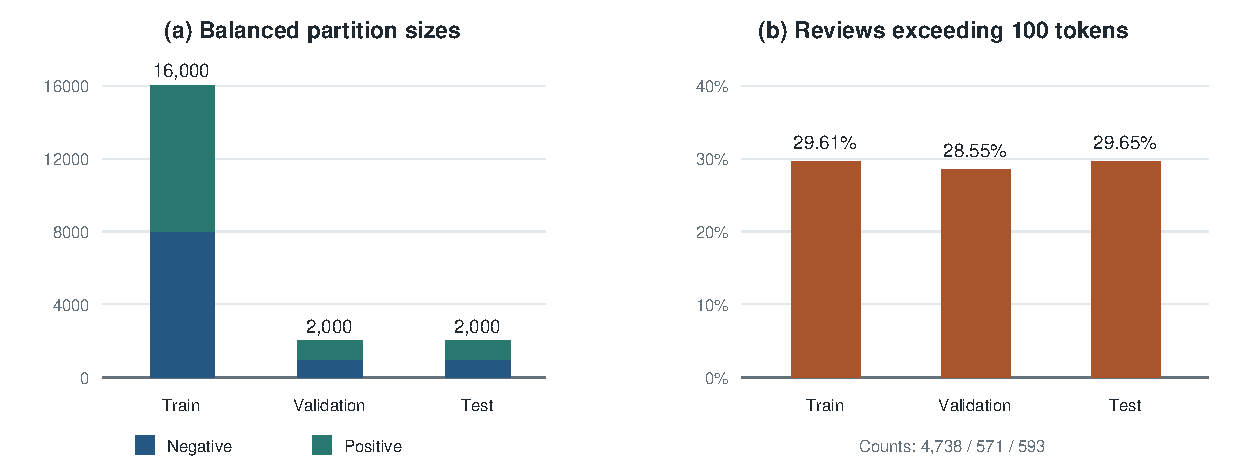
\includegraphics[width=0.80\textwidth]{figures/dataset_coverage.pdf}
\caption{Dataset allocation and sequence coverage from the saved data audit and sequence metadata. Every partition is class-balanced. The right panel measures reviews whose tokenized length exceeds the shared 100-token sequence limit; the MLP has no corresponding token-prefix restriction.}
\label{fig:coverage}
\end{figure*}

Figure~\ref{fig:coverage} quantifies coverage across all partitions. The training and validation truncation rates are 29.61\% and 28.55\%, respectively, compared with 29.65\% on test reviews. The restriction is therefore relevant throughout model fitting and selection, rather than arising only during final evaluation. These percentages count affected reviews; they do not measure how many words are lost or establish that the omitted words are decisive.

The 50\% majority-class reference accuracy follows directly from the balanced test composition. This reference is useful for interpreting classification performance, but it does not describe a deployed review stream in which polarity prevalence might differ. No claim about real-world sentiment prevalence follows from a deliberately balanced sample. In particular, precision measured here need not transfer unchanged to an application with a different ratio of positive to negative reviews.


\subsection{Validation-Based Tuning and Evaluation}
Every architecture uses the same two-candidate search: dropout 0.3 with learning rate $10^{-3}$, and dropout 0.5 with learning rate $5\times10^{-4}$. Batch size is 32, the maximum training budget is eight epochs per candidate, and early stopping monitors validation loss with patience two. The lowest-validation-loss checkpoint is retained. Candidate selection is based solely on validation loss; the fixed test set is evaluated after all candidate selections are complete. Table~\ref{tab:selected} reports the selected settings and stopping outcomes.

\begin{table*}[tbp]
\fontsize{9}{10.2}\selectfont
\centering
\caption{Validation-Selected Configurations and Training Outcomes}
\label{tab:selected}
\setlength{\tabcolsep}{7pt}\renewcommand{\arraystretch}{1.12}
\begin{tabular}{lccccc}
\toprule
Model & Dropout & Learning rate & Best val. loss & Epochs run & Best epoch \\ \midrule
MLP & 0.5 & $5\times10^{-4}$ & 0.2627 & 3 & 1 \\
TextCNN & 0.3 & $10^{-3}$ & 0.2969 & 4 & 2 \\
BiLSTM & 0.3 & $10^{-3}$ & 0.2802 & 3 & 1 \\
\bottomrule
\end{tabular}
\end{table*}

Accuracy is computed across both classes. Precision, recall, and F1-score are reported for the positive class. For true positives (TP), true negatives (TN), false positives (FP), and false negatives (FN),
\begin{align}
\mathrm{Accuracy}&=\frac{\mathrm{TP}+\mathrm{TN}}{\mathrm{TP}+\mathrm{TN}+\mathrm{FP}+\mathrm{FN}},\\
\begin{split}
\mathrm{Precision}&=\frac{\mathrm{TP}}{\mathrm{TP}+\mathrm{FP}},\quad
\mathrm{Recall}=\frac{\mathrm{TP}}{\mathrm{TP}+\mathrm{FN}},\\
\mathrm{F1}&=\frac{2\,\mathrm{Precision}\,\mathrm{Recall}}{\mathrm{Precision}+\mathrm{Recall}}.
\end{split}
\end{align}
Both-class reports, confusion matrices, and all per-review predictions are also retained. A single random seed is used; no multi-seed mean, confidence interval, or significance test is claimed.


\subsection{Selection controls and reproducibility}
The two candidate settings change dropout and learning rate together. Accordingly, the experiment estimates the behavior of two configuration bundles, not the isolated causal effect of either regularization or learning rate. An eight-epoch upper bound is identical across candidates, but early stopping permits different actual epoch counts. A model trained for three epochs and one trained for four epochs have equal maximum opportunity under this rule, not equal realized computation.

The reproducibility sequence is: (1) pin the source revision and sampling seed; (2) save review identities and split assignments; (3) fit and save training-only representations; (4) train each candidate and retain its minimum-validation-loss checkpoint; (5) compare candidates using that loss; and (6) evaluate the selected checkpoints with the same fixed threshold. Candidate histories document the optimization trajectory, while confusion matrices and per-review outputs support reconstruction of the reported classification scores.

The source signature and artifact hashes help detect accidental reuse of incompatible cached stages. They do not themselves establish scientific correctness: the interpretation also depends on the declared partition semantics, the absence of information leakage, and the meaning of the label. A single seed documents one realized experiment and does not quantify variation across repeated sampling and optimization.


\subsection{Implementation and Memory Use}
The implementation uses Python 3.12, TensorFlow 2.21.0, Keras 3.15.1, NumPy 2.5.4, and scikit-learn 1.9.1. Training and inference ran on a local CPU; TensorFlow reported no usable GPU device. Each heavy preparation, candidate-training, and selected-model evaluation stage runs in a separate process, releasing its allocations when complete. Dataset prefetching and CPU-thread use are bounded, and sequence arrays are memory-mapped.

Only the selected review strings are assembled into pandas data frames. TF-IDF remains sparse until a batch is consumed by the MLP. The 16,000-by-20,000 training feature matrix occupies 10,634,684 bytes in CSR form, compared with 2,560,000,000 bytes for a full float64 dense representation, a reduction of approximately 241 times in feature-storage size. A dense float32 batch of 32 reviews requires approximately 2.44 MiB. These figures concern feature storage, not the entire training process.

The largest recorded worker-process-tree private memory was 686.5 MiB, sampled approximately once per second during data preparation. The summed duration of the 12 isolated stages was 818.78 seconds on this machine. Source hashes, dataset revision, split identifiers, package versions, histories, checkpoints, and resource measurements are preserved. Nine regression tests and 38 independent result checks passed, including checks for split overlap and recomputation of metrics from saved predictions.


\begin{figure*}[tbp]
\centering
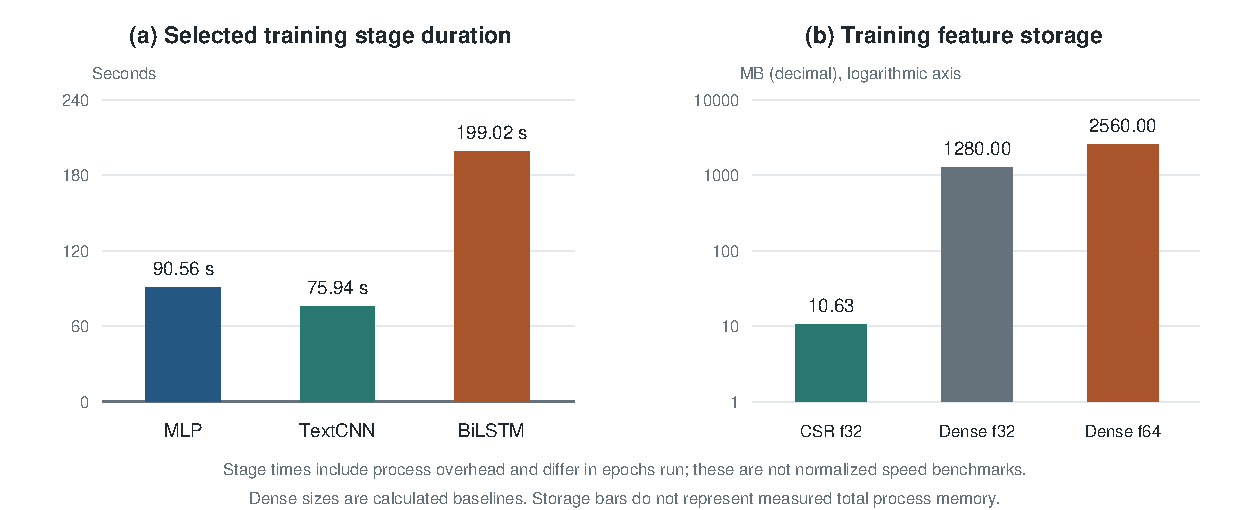
\includegraphics[width=0.80\textwidth]{figures/resource_comparison.pdf}
\caption{Recorded duration of the selected candidate-training stages and calculated training feature storage. The stage times are 90.56, 75.94, and 199.02 seconds for MLP, TextCNN, and BiLSTM. Dense float32 and float64 sizes are arithmetic baselines, not measured allocations; storage uses decimal MB on a logarithmic axis.}
\label{fig:resources}
\end{figure*}

Figure~\ref{fig:resources} puts storage and execution cost in context. Holding precision constant, the hypothetical dense float32 matrix would occupy 1.28 GB, approximately 120 times the recorded CSR storage. The approximately 241-fold comparison with dense float64 additionally includes a factor of two from numeric precision. The training matrix has 1,321,335 nonzero entries among 320 million possible entries, a density of approximately 0.413\%. Sparse storage is therefore useful because most review--term combinations are absent.

The selected training stages include worker startup and related stage overhead. Their durations are distinct from the internal fitting durations of 80.78, 64.83, and 190.31 seconds recorded in the selected-model summaries. BiLSTM's stage takes approximately 2.62 times the TextCNN stage duration on this CPU, despite similar parameter counts and fewer epochs run. This is an observed implementation cost, not a hardware-independent ratio or a normalized per-epoch benchmark. No latency or energy-efficiency claim is made.


\section{Results and Discussion}
\subsection{Common Test-Set Comparison}
Table~\ref{tab:results} presents the common comparison on the 2,000 held-out reviews. The MLP achieves the highest accuracy and positive-class F1-score in this run. Its 88.20\% accuracy exceeds BiLSTM by 2.10 percentage points and TextCNN by 2.80 percentage points. The absolute differences should be interpreted within this single split, seed, representation choice, and small tuning grid.

\begin{table*}[tbp]
\fontsize{9}{10.2}\selectfont
\centering
\caption{Test Performance on the Common 2,000-Review Partition}
\label{tab:results}
\renewcommand{\arraystretch}{1.15}\setlength{\tabcolsep}{12pt}
\begin{tabular}{lrrrr}
\toprule
Model & Accuracy (\%) & Precision & Recall & F1-score \\ \midrule
MLP (TF-IDF) & \textbf{88.20} & \textbf{0.8760} & \textbf{0.8900} & \textbf{0.8829} \\
TextCNN & 85.40 & 0.8371 & 0.8790 & 0.8576 \\
BiLSTM & 86.10 & 0.8588 & 0.8640 & 0.8614 \\
\bottomrule
\end{tabular}
\end{table*}

The MLP correctly classifies 874 negative and 890 positive reviews, making 126 false-positive and 110 false-negative predictions. TextCNN produces 171 false positives and 121 false negatives, whereas BiLSTM produces 142 and 136, respectively. TextCNN's relatively higher recall than BiLSTM is accompanied by lower precision, reflecting more negative reviews classified as positive. These differences provide a more informative account than accuracy alone.


\begin{figure*}[tbp]
\centering
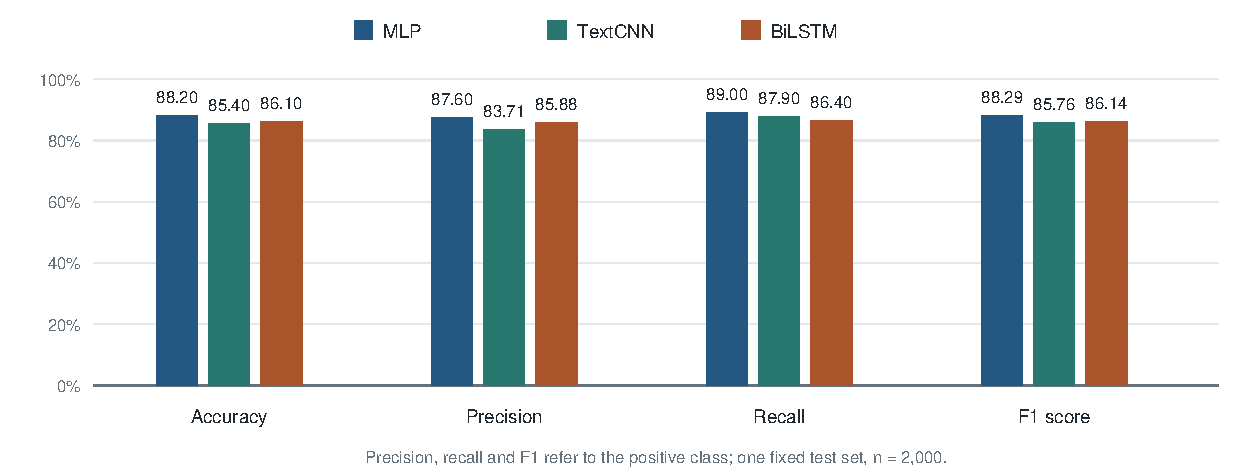
\includegraphics[width=0.80\textwidth]{figures/metric_comparison.pdf}
\caption{Common test-set metrics for the three selected configurations. All axes start at zero; precision, recall, and F1 are positive-class measures. Values are percentages for visual comparison, with exact proportions reported in Table~\ref{tab:results}. No repeated-run uncertainty is estimated.}
\label{fig:metrics}
\end{figure*}

\begin{figure*}[tbp]
\centering
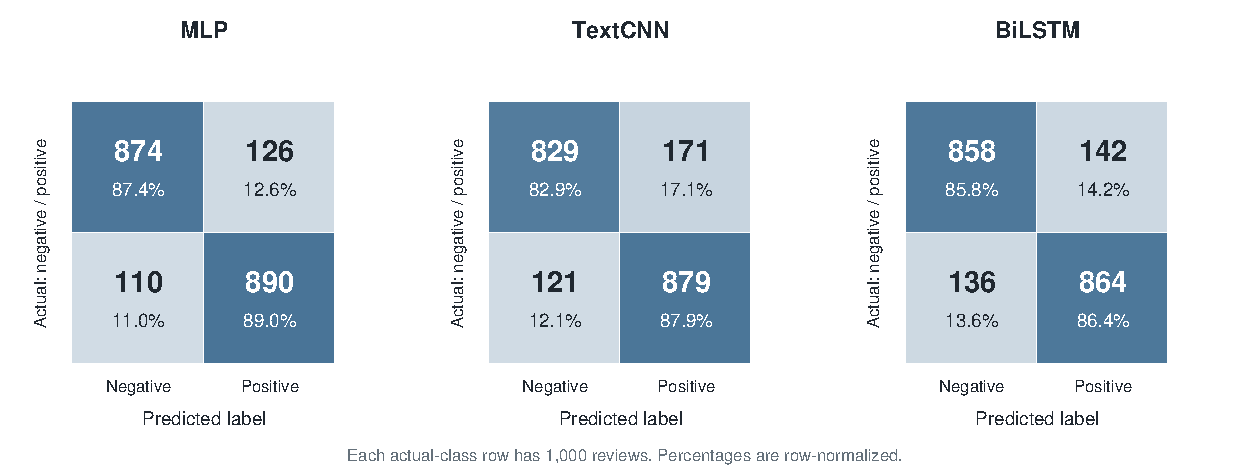
\includegraphics[width=0.80\textwidth]{figures/confusion_matrices.pdf}
\caption{Confusion matrices on the same 2,000 test reviews. Rows denote actual labels and columns denote predicted labels. Counts and percentages within each actual class are shown; each row has 1,000 reviews.}
\label{fig:confusions}
\end{figure*}

Figures~\ref{fig:metrics} and~\ref{fig:confusions} show that the ranking is not explained by a single aggregate number. MLP correctly recognizes 87.4\% of negative reviews and 89.0\% of positive reviews. The corresponding negative-class recognition rates are 82.9\% for TextCNN and 85.8\% for BiLSTM. Because class supports are equal, accuracy is numerically equal to the average of the positive and negative recall rates in this test partition.

At the fixed threshold, the predicted-positive counts are 1,016 for MLP, 1,050 for TextCNN, and 1,006 for BiLSTM. TextCNN's 52.5\% predicted-positive share, compared with 50\% actual positives, is consistent with its larger false-positive count. This diagnostic describes the operating point of the chosen threshold. It is not a probability-calibration assessment, since calibration requires comparing predicted probabilities with observed frequencies over probability ranges.

MLP makes 42 fewer errors than BiLSTM and 56 fewer than TextCNN on these 2,000 reviews. The error reductions relative to those models are approximately 15.1\% and 19.2\%, respectively. These are descriptive comparisons of counts from the same test set; they do not establish statistical significance or predict the improvement on another sample. Any threshold adjustment for an application with asymmetric error costs should use validation data and a prespecified operating requirement.


\subsection{Training Dynamics and Architectural Interpretation}
Figure~\ref{fig:loss} shows loss trajectories for the selected configurations. MLP and BiLSTM reach their lowest validation loss after the first epoch; TextCNN reaches it after the second. Continued training reduces training loss while increasing validation loss. The retained checkpoints therefore precede the final fitted epochs. Early stopping limits continued fitting after validation deterioration, but does not establish that overfitting has been eliminated.

\begin{figure*}[tbp]
\centering
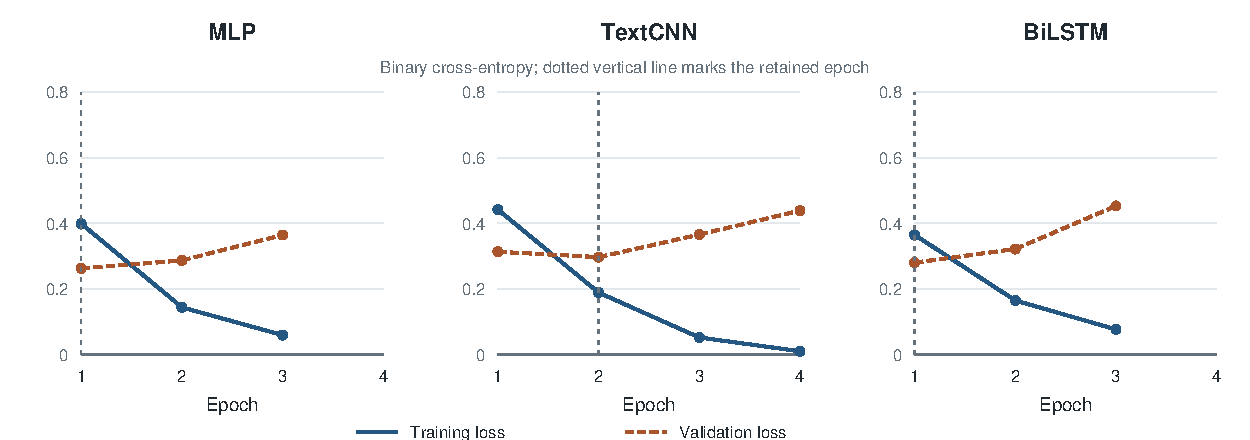
\includegraphics[width=0.80\textwidth]{figures/training_curves.pdf}
\caption{Training and validation cross-entropy for the selected configurations. Training loss is averaged during parameter updates, whereas validation loss is measured after an epoch; their levels are not a direct comparison of one fixed model. Best checkpoints occur at epochs 1, 2, and 1 for MLP, TextCNN, and BiLSTM, respectively.}
\label{fig:loss}
\end{figure*}

The MLP's lexical representation provides a plausible explanation for its strong performance on this subset: frequent sentiment-bearing words and bigrams can be informative without requiring a sequence encoder to learn useful embeddings from 16,000 reviews. Its features also cover the complete review. The result is consistent with the importance of efficient lexical baselines discussed by Joulin et al.~\cite{joulin2017}; it does not imply that TF-IDF is preferable under all data regimes.

TextCNN can detect local expressions, but global max pooling emphasizes strong local activations without explicitly modeling a review's final overall judgment. BiLSTM preserves order within the observed sequence and performs better than TextCNN here, but its increased sequential modeling capacity does not overcome the MLP under this protocol. Neither architectural property proves the cause of an individual prediction. Limited training data, randomly initialized embeddings, truncation, optimization, and the search budget can all influence the ranking.


\subsection{Shared errors and disagreement}
\begin{figure*}[tbp]
\centering
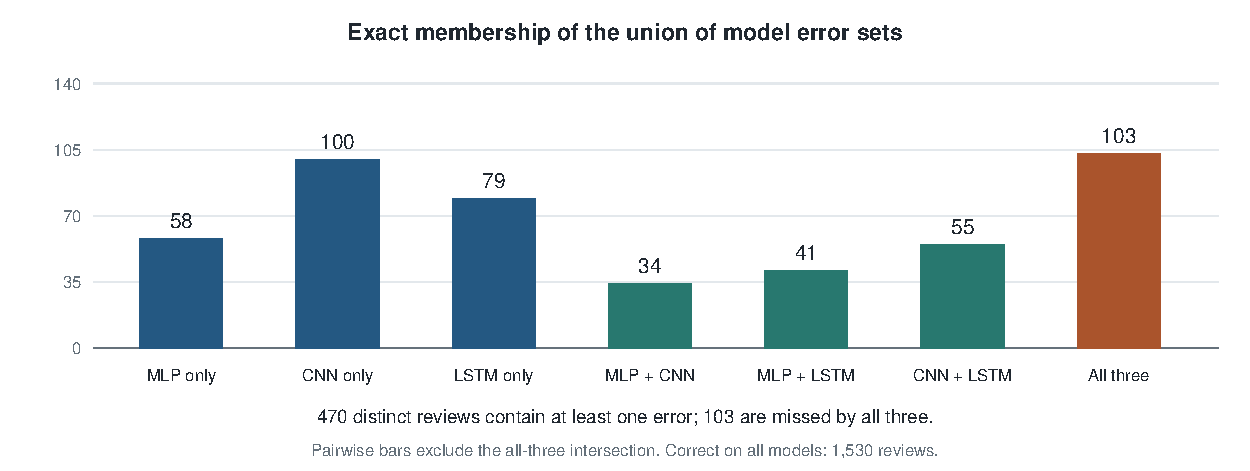
\includegraphics[width=0.80\textwidth]{figures/error_overlap.pdf}
\caption{Exact, mutually exclusive intersections of the three misclassification sets, computed from saved source review identifiers. A pairwise bar excludes reviews missed by all three. The seven bars sum to the 470-review error union; their memberships reconstruct each model's error count.}
\label{fig:overlap}
\end{figure*}

Figure~\ref{fig:overlap} distinguishes complementary mistakes from errors shared across architectures. The 103 reviews missed by all three constitute 21.9\% of the union of error sets and 5.15\% of the full test set. Conversely, all three classify 1,530 reviews correctly. Agreement across architectures is therefore common, but agreement alone does not establish that the source label is semantically unambiguous.

The remaining error memberships identify cases on which at least one model succeeds while another fails. This complementarity motivates inspecting disagreements, rather than interpreting each architecture through only its most confident errors. It also suggests a possible ensemble investigation. The present experiment does not train or validate an ensemble, so the union and intersection counts must not be presented as an achieved ensemble score.

The relationship between training and validation loss further limits interpretation. Training loss is accumulated while parameters change and dropout is active; validation loss is calculated after the epoch without training-time dropout. A lower validation loss than the first-epoch training average can therefore occur without contradicting the data split. The later increase in validation loss, alongside falling training loss, is the relevant warning of deteriorating generalization in these histories.


\subsection{Observed Failure Cases}
The selected MLP, TextCNN, and BiLSTM misclassify 236, 292, and 278 test reviews, respectively. All three misclassify 103 of the same source reviews; the union of their error sets contains 470 reviews. A targeted qualitative review examines nine real source reviews, preserving all three predictions. It is not a random annotated sample and cannot estimate the prevalence of linguistic error categories.

\textit{Negation and changing context:} Source review 3,258,943 is positively labeled and titled ``Not bad after rebate,'' but all models predict negative. The text combines a favorable qualified assessment with criticism of video speed. In review 191,582, earlier remedies failed while the reviewed product improved the problem and is recommended. All three models again predict negative. These examples distinguish the scope and target of negative expressions from the presence of a negative word alone.

\textit{Mixed sentiment and opinion targets:} Review 317,569 initially praises a clock's automatic setting but later describes an excessively bright display and a failed alarm. MLP and BiLSTM predict positive despite the negative label; TextCNN predicts negative. In review 58,355, a ``horrible sequel'' is criticized while the reviewed classic in high definition is praised. TextCNN predicts negative, whereas MLP and BiLSTM predict positive. Correct classification requires distinguishing opinions about related objects rather than aggregating all evaluative expressions indiscriminately.

\textit{Ironic praise:} Review 1,876,833 calls an expensive toy ball an ``excellent deal'' but concludes that the writer will pass on buying it. The praise is plausibly ironic in context. TextCNN and BiLSTM predict positive, while MLP predicts negative. Review 2,059,653 describes most album tracks as unlistenable and jokes that they improve when the skip button is used, while praising two tracks; all models predict positive despite the negative label. These cases indicate difficulties with contextual reversal, without establishing a general sarcasm-detection capability for any architecture.

\textit{Domain wording, language, and label consistency:} All models predict negative for review 1,934,203, where ``sucks'' describes successful dust removal and most of the review is favorable. A negatively worded Spanish album review, source row 756,579, is classified as positive by all three models, illustrating a limitation of the shared ASCII-oriented preprocessing and learned representations. Finally, review 2,005,780 has a positive source label but explicitly rejects the game and suggests awarding zero stars; all models predict negative. This is a suspected label--text conflict, not a confirmed semantic model failure. The original label remains unchanged and the row remains an error in every reported score.

The automatic review aids flag 1,352 test reviews with negation cues, 220 with mixed word-polarity cues, and 18 with possible-sarcasm cues. The groups overlap. The toy-ball example is missed by the simple sarcasm phrase list, while an ordinary use of ``as if'' can be flagged. These counts therefore describe heuristic subsets, not verified linguistic categories or measured sarcasm prevalence. The observed texts support qualitative hypotheses; no causal feature-attribution experiment is reported.


\begin{table*}[tbp]
\fontsize{9}{10.2}\selectfont
\centering
\caption{Qualitative Review of Selected Source Cases}
\label{tab:cases}
\renewcommand{\arraystretch}{1.10}\setlength{\tabcolsep}{4pt}
\begin{tabularx}{\linewidth}{@{}P{19mm}P{18mm}P{28mm}Y@{}}
\toprule
Source row & Label & Predictions M/C/B & Interpretation requiring review \\ \midrule
3,258,943 & Positive & Neg / Neg / Neg & Qualified praise and criticism appear together; negative words do not alone determine the intended polarity. \\
317,569 & Negative & Pos / Neg / Pos & Initial praise is reversed by display and alarm failures. \\
58,355 & Positive & Pos / Neg / Pos & Criticism of a related sequel differs from praise for the reviewed work. \\
1,876,833 & Negative & Neg / Pos / Pos & Apparently favorable price language is plausibly ironic in the full context. \\
756,579 & Negative & Pos / Pos / Pos & Spanish wording exposes the limits of preprocessing and learned representations. \\
2,005,780 & Positive & Neg / Neg / Neg & Explicit rejection conflicts with the positive source label; the label remains unchanged. \\
\bottomrule
\end{tabularx}
\par\vspace{3pt}{\footnotesize M/C/B denote MLP, TextCNN, and BiLSTM. Cases are selected examples, not a prevalence sample.}
\end{table*}

Table~\ref{tab:cases} condenses six of the nine reviewed cases while the surrounding discussion retains their context. A text can support several interpretations simultaneously: mixed opinions can involve a change of target, and an apparent failure of negation handling can also reflect an omitted conclusion. The review does not force these possibilities into mutually exclusive causal labels. Resolving the cause would require inspecting the actual input prefix, conducting controlled text edits, or using a separately specified explanation method.

The suspected label conflict deserves separate treatment. A classifier can disagree with the stored label while aligning with a reasonable human reading; conversely, human readers can disagree about an ambiguous review. Keeping the original label in the metric calculation preserves comparability and avoids changing evaluation rules after observing errors. A future annotation study could record independent judgments and adjudication without silently revising the current benchmark.


\begin{table*}[tbp]
\fontsize{9}{10.2}\selectfont
\centering
\caption{Controlled Follow-Up Experiments}
\label{tab:future}
\renewcommand{\arraystretch}{1.10}\setlength{\tabcolsep}{4pt}
\begin{tabularx}{\linewidth}{@{}P{30mm}P{54mm}Y@{}}
\toprule
Question & Controlled change & Evidence to collect \\ \midrule
Does model ordering persist? & Prespecify repeated seeds and apply the same search budget to every model. & Per-seed scores and variability; retain paired predictions. \\
Does input coverage affect ranking? & Compare full and matched-prefix TF-IDF with several prespecified sequence limits. & Validation-selected lengths and a fresh held-out comparison. \\
Does padding influence TextCNN? & Change padding treatment while fixing reviews, tokenizer, filters, and tuning budget. & Loss curves, scores, and short-review behavior. \\
Can contextual representations help? & Introduce pretrained embeddings or a Transformer baseline with a declared compute budget. & Accuracy, error overlap, memory, and runtime under the new protocol. \\
Which linguistic errors recur? & Independently annotate a random review sample with a documented rubric. & Annotator agreement and category-specific counts with denominators. \\
\bottomrule
\end{tabularx}
\end{table*}

\subsection{Limitations}
The study is restricted to one balanced subset, one random seed, and two configurations per architecture. It provides neither repeated-run variability nor a statistical significance claim. The MLP and sequence models differ in input representation and access to later tokens, and pretrained word vectors are not evaluated. The labeled corpus includes multilingual text and potential label ambiguity that the binary protocol does not resolve. The nine reviewed examples are selected from observed failures, so their category frequencies must not be generalized to the complete test set. The reported memory and timing measurements are specific to this implementation and CPU environment.


The balanced sample is small relative to the source corpus and does not establish product-category generalization. Splitting reviews does not necessarily separate products, authors, or closely related descriptions, so the study does not claim a product-disjoint or author-disjoint evaluation. The no-overlap checks cover source row identity and exact cleaned text; they do not prove the absence of semantic near duplicates.

The fixed threshold provides a transparent common operating point but does not establish calibration, robustness to changed class prevalence, or suitability for an application with unequal error costs. Error categories generated by cue lists are particularly limited: overlapping cue counts cannot be converted into disjoint linguistic frequencies, and a cue's presence does not establish why a network failed. These threats bound the interpretation of both quantitative and qualitative findings.


\section{Conclusion}
Under a common balanced Amazon Polarity protocol, the TF-IDF MLP achieves the strongest observed test performance, with 88.20\% accuracy and a positive-class F1-score of 0.8829. BiLSTM reaches 86.10\% accuracy, followed by TextCNN at 85.40\%. The findings demonstrate that a feed-forward classifier using informative lexical features can remain competitive with convolutional and recurrent architectures when labeled data and tuning budgets are limited. Full-review feature coverage is an additional advantage of the MLP in this particular design, so the ranking should not be attributed exclusively to architecture.

Validation-based checkpoint selection avoids evaluating later epochs after validation loss deteriorates, and a memory-conscious implementation enables the real-data experiment to complete locally. The reviewed failures show that negation scope, changing opinion targets, mixed sentiment, and ironic language remain challenging across models. Suspected label inconsistency further limits a literal interpretation of every disagreement with the dataset label. These conclusions are bounded by the single-seed protocol and the observed configurations.

\section{Future Work}
Future experiments should repeat training across prespecified seeds and report variability before drawing stronger conclusions about model ordering. Longer sequence limits, matched text coverage, and pretrained embeddings would help separate representation effects from architecture effects. Attention-based recurrent encoders~\cite{zhou2016} and pretrained Transformers~\cite{vaswani2017,devlin2019} provide further comparison points, subject to a comparable validation and compute budget.

Unicode-preserving preprocessing and explicit evaluation by review language could address limitations exposed by multilingual examples. A separately annotated, randomly sampled error set would support more reliable analysis of negation, mixed sentiment, sarcasm, and label ambiguity. Such refinements should be designed using training and validation data, or a new evaluation protocol, rather than selected retrospectively to improve the present test scores.




Table~\ref{tab:future} turns the observed limitations into falsifiable follow-up questions. Each proposed change requires a declared comparison protocol rather than retrospective modification of the current test set. The matched-prefix TF-IDF experiment is especially useful because it changes text coverage while retaining the feed-forward classifier family. A separate length comparison for the sequence models would then examine the interaction between coverage and sequential encoding.

For eventual use in review monitoring, an additional temporal evaluation should examine newly collected reviews with a documented source and label policy. Vocabulary, product mix, and class prevalence may differ from the balanced development sample. Monitoring should distinguish changes in input distribution from verified changes in prediction quality. These deployment-oriented evaluations remain proposed work and are not outcomes of the present study.


\section*{Acknowledgement}
\phantomsection
\addcontentsline{toc}{section}{Acknowledgement}
The authors acknowledge the publicly available Amazon Polarity dataset and the open-source TensorFlow/Keras, scikit-learn, and Hugging Face software used to implement and evaluate the project.
